\section[Общая схема протокола]{Общая идея релятивистского квантового распределения ключей через открытое пространство без синхронизации часов}
\begin{itemize}
  \item Алиса и Боб контролируют области пространства, необходимые для приготовления и измерения протяженных квантовых состояний.
  \item Расстояние $L$ между Алисой и Бобом всем известно и является параметром протокола. Алиса и Боб имеют часы, но не имеют общего начала отсчета времени (часы не синхронизированы).
  \item Происходит передача серии состояний Алисой. Каждая посылка происходит в случайный момент времени внутри интервала $\Delta T$. 
  Достаточно, чтобы Алиса случайно выбирала один из двух моментов посылки сигнала внутри интервала $\Delta T$ (рис \ref{fig:timeline}). 
  Алиса готовит протяженное классическое состояние, состоящее из пары интенсивных когерентных пакетов, разделенных интервалом $l > l_{pac}$ ($l_{pac}$~--- ширина пакета, см. ниже): 
  $|\alpha_c\rangle_1 \otimes|\alpha_c\rangle_2$ (индексы <<1>> и <<2>> отвечают пакетам, локализованным в моменты времени 1 и 2, рис \ref{fig:process}); среднее число фотонов в состоянии $\mu_c = |\alpha_c|^2 \gg 1$. 
  Временное разрешение проводится с точностью до ширины пакета $l_{pac}$ (интервалы времени, меньшие $l_{pac} / c$, считаются нулевыми). 
  Момент времени $t_{A,i}$ посылки состояния в канал связи Алисой фиксируется по своим часам.
  
  \begin{figure}[h]
  \center{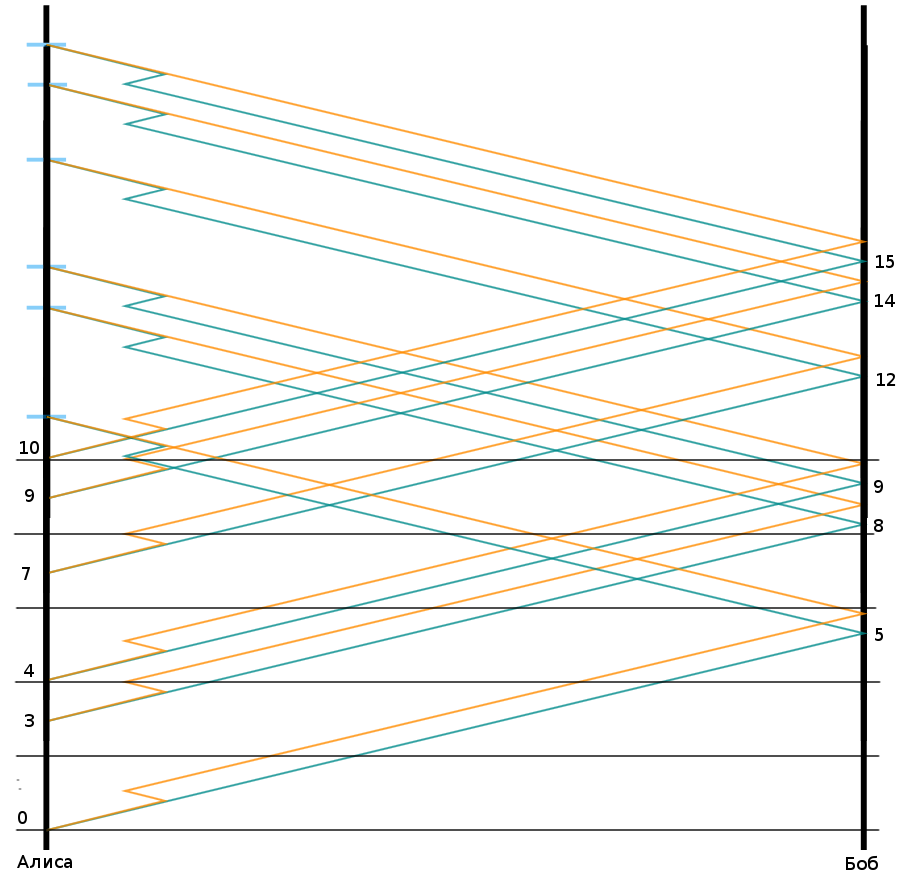
\includegraphics[width=0.9\linewidth]{timeline}}
  \caption{Пространственно-временная диаграмма, поясняющая посылку классических и прием квантовых состояний в случайные моменты. Слева и справа с помощью <<0>> и <<1>> обозначены моменты посылки и приема состояния}
  \label{fig:timeline}
  \end{figure}
  \begin{figure}[h]
  \center{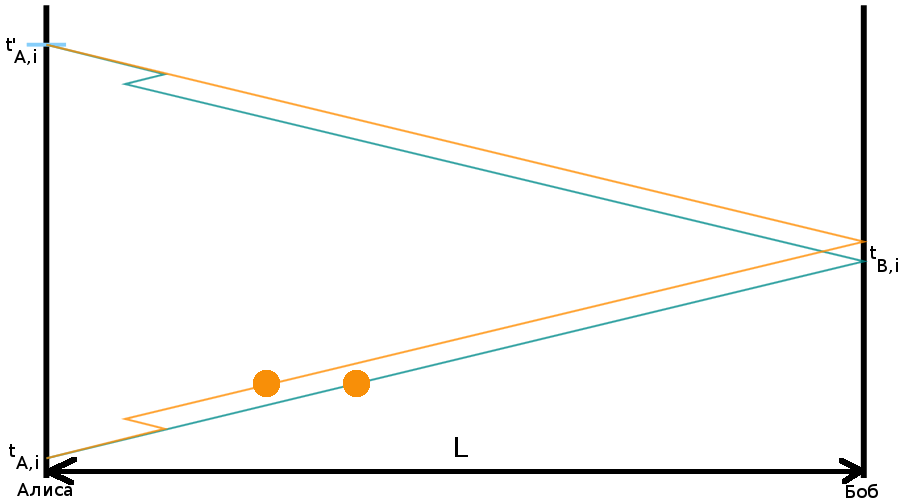
\includegraphics[width=0.9\linewidth]{not_catched}}
  \caption{Пространственно-временная диаграмма, поясняющая процесс приготовления, преобразования и распространения протяженных квантовых состояний}
  \label{fig:process}
  \end{figure}
  \begin{figure}[h]
  \center{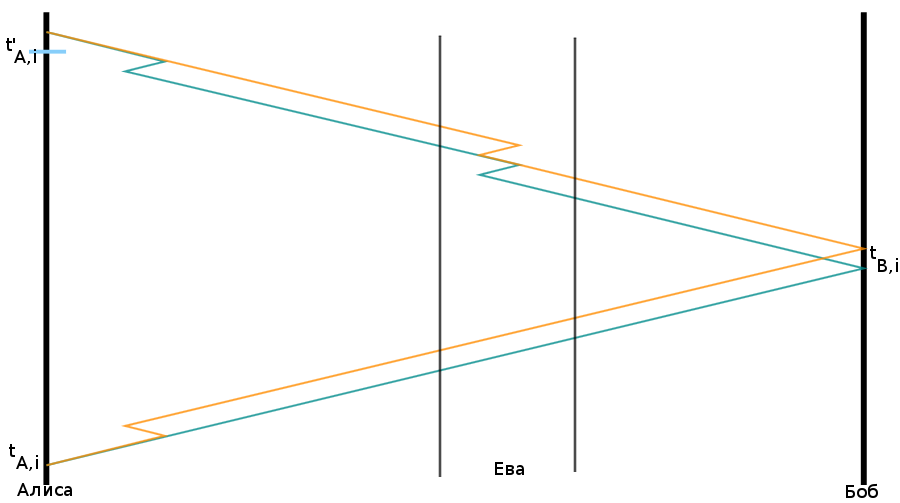
\includegraphics[width=0.9\linewidth]{eve_detected}}
  \caption{Пространственно-временная диаграмма, поясняющая причину задержек по времени протяженных состояний при подслушивании Евой}
  \label{fig:detected}
  \end{figure}
  
  \item Аппаратура Боба на приемной стороне работает в ждущем режиме. При помощи быстрого классического детектора Боб фиксирует момент прихода состояния в каждой $i$-й посылке $t_{B,i}$. 
  Далее классический сигнал ослабляется до квазиоднофотонного уровня, и при помощи фазового модулятора на одну из <<половинок>> (заднюю) случайным образом навешивается фаза. 
  Состояние $|\alpha\rangle_1 \otimes |e^{i\varphi_B}\alpha\rangle_2$ ($\mu = |\alpha|^2 < 1$) направляется обратно к Алисе 
  \footnote{Все задержки на стороне Боба, связанные с обработкой, заранее известны. Их величина непринципиальна и считается включенной в моменты $t_{A,B,i}$ и $t'_{A,B,i}$.}. 
  Значение относительной фазы у двух импульсов $\varphi_B = \varphi_0$ отвечает выбору логического 0 в ключе, а $\varphi_B = \varphi_1$~--- логической 1. 
  Кодирование осуществляется на стороне Боба.
  
  \item Алиса, зная расстояние $L$ и время отправки $t_{A,i}$ по своим часам своего состояния в канал связи, знает время прихода квантового состояния от Боба $t'_{A,i}$, преобразует состояния, случайно и независимо от Боба изменяет относительную фазу одной из <<половинок>>: 
  $|\alpha\rangle_1 \otimes |e^{i\varphi_B}\alpha\rangle_2 \rightarrow |\frac{\alpha}{2}\rangle_1 \otimes |\frac{(e^{i\varphi_B} - e^{i\varphi_A})\alpha}{2}\rangle_2$
  ($\varphi_A = \varphi_0$ или $\varphi_A = \varphi_1$), и производит измерения \textit{только в определенном временном окне}. 
  Если $\varphi_A \neq \varphi_B$, то возникает отсчет в детекторе, а если $\varphi_A = \varphi_B$, то отсчета не возникает. В результате Алиса знает, какой бит ключа посылал Боб.
  
  \item После проведения серии посылок Боб сообщает Алисе интервалы времени между соседними посылками (рис \ref{fig:timeline}), которые он фиксировал по своим часам. Алиса сравнивает их со своими интервалами времени между посылками по своим часам. Подсчитывается доля их несовпадений $\eta$. Соседние посылки, интервалы между которыми не совпали, Алиса и Боб отбрасывают.
  
  \item Далее часть последовательности Алисой и Бобом раскрывается и сравнивается для оценки вероятности ошибки. Если ошибка меньше критической, то происходит исправление ошибок через открытый классический канал связи. Затем происходит сжатие очищенного ключа. В результате возникает секретный ключ, известный только Алисе и Бобу.
\end{itemize}

Отметим, что Алиса и Боб не должны следить за средним числом долетевших посылок. Потери в канале связи, как будет показано позднее, вообще не входят в критерий секретности ключей.
\clearpage